\documentclass[12pt,a4paper]{report}

\usepackage[utf8]{inputenc}
\usepackage{amsmath, amsfonts, amssymb}
\usepackage{graphicx}
\usepackage{float}
\usepackage{subcaption}
\usepackage{booktabs}
\usepackage{tikz}
\usetikzlibrary{shapes.geometric, arrows.meta, positioning}
\usepackage{hyperref}
\usepackage[left=3.8cm, right=2.5cm, top=2.5cm, bottom=2.5cm]{geometry}
\usepackage{natbib}
\usepackage{mathptmx} % Times New Roman font
\usepackage{setspace}
\usepackage{indentfirst} % Forces indent on first paragraph after heading
\onehalfspacing

% --- Chapter Title Formatting ---
\usepackage{fmtcount} % Allows numbers to be spelled out (e.g. ONE)
\usepackage{titlesec}

% \large is exactly 14.4pt when the base font is 12pt
\titleformat{\chapter}[display]
  {\centering\normalfont\large\bfseries} % Center alignment, 14pt (large), Bold
  {\MakeUppercase{\chaptertitlename}\ \thechapter} % Prints "CHAPTER 1"
  {1\baselineskip} % Space between "CHAPTER 1" and the title
  {\MakeUppercase} % Formats the actual title text (e.g., INTRODUCTION)
\titlespacing*{\chapter}{0pt}{-20pt}{1.5cm} % Pull up to top margin, gap after

% \normalsize is exactly 12pt when the base font is 12pt
\titleformat{\section}
  {\normalfont\normalsize\bfseries} % 12pt, Bold
  {\thesection}
  {1.27cm} % Matches the 0.5 inch tab indent
  {}
\titlespacing*{\section}{0pt}{1.5\baselineskip}{0pt}

\titleformat{\subsection}
  {\normalfont\normalsize\bfseries} % 12pt, Bold
  {\thesubsection}
  {1.27cm}
  {}
\titlespacing*{\subsection}{0pt}{1.5\baselineskip}{0pt}

\titleformat{\subsubsection}
  {\normalfont\normalsize\bfseries\itshape} % 12pt, Bold, Italic
  {\thesubsubsection}
  {1.27cm}
  {}
\titlespacing*{\subsubsection}{0pt}{1.5\baselineskip}{0pt}
% --------------------------------

\setlength{\parindent}{1.27cm} % Exactly 0.5 inch indent for paragraphs

\title{\textbf{Uncovering Parent Profiles Through Cluster Analysis for Targeted Virtual Counseling} \\ \vspace{0.5cm} \Large Master by Research Proposal}
\author{Statistics Faculty Candidate}
\date{\today}

\begin{document}

\pagenumbering{roman}

\maketitle

\tableofcontents
\clearpage

\pagenumbering{arabic}
\chapter{Introduction}

\section{Background of the Study}
A defining characteristic of the global counselling landscape is the rapid transition to Digital Health Interventions (DHIs) for delivering psychological programs \citep{Wind2020_98, Naslund2017_76, Sutherland2018_77}. Traditional in-person counselling often presents insurmountable barriers for caregivers of children with Autism Spectrum Disorder (ASD), including high financial costs, severe time constraints, and logistical challenges. To democratize access to mental health support, international counselling programs increasingly utilize asynchronous e-learning, real-time videoconferencing, and mobile health (mHealth) applications to deliver targeted therapy. 

In Malaysia, the drive toward targeted counselling through specialized frameworks is not merely a clinical preference but a systemic necessity. The prevalence of ASD in Malaysia mirrors the global surge \citep{Santomauro2025_73}. However, the Malaysian experience is filtered through a complex lens of cultural stigma, varying socio-economic status, and a centralized healthcare system that often struggles with "one-size-fits-all" support models. For many Malaysian caregivers, spiritual coping and communal support (the "Kampung Spirit") are as vital as clinical psychotherapy. A critical analysis suggests that targeted counselling in Malaysia is only effective if data-driven groupings include these specific cultural belief systems as clustering indicators. 

\section{Problem Statement}
With a global pediatric prevalence of 0.77\%, Malaysian researchers face a persistent challenge with under-reporting in rural regions. Critically, the lack of a mandatory national registry for neurodivergence creates a "data shadow," where many families remain outside the reach of data-driven interventions. This creates a bifurcation in the caregiver population: urban families with access to private, data-rich interventions, and rural families relying on generalized, often outdated public support. 

Furthermore, the "Oxygen Mask Principle" faces a harsh reality in the Malaysian public sector. With a specialist-to-patient ratio that remains below recommended international levels, the caregiver burden is exacerbated by long wait times for diagnosis and intervention. When a parent's psychological health is compromised, it hinders the child's trajectory \citep{Rusu2025_94, SnchezAmate2024_95, Palmer2020_83}. In Malaysia, this creates a vicious cycle where the lack of targeted support for the parent leads to developmental plateauing in the child, further increasing the caregiving load. Ignoring the heterogeneity of these caregivers and forcing them into standardized counseling programs invariably leads to high attrition rates \citep{Wang2025_74, Liu2025_72}.

\section{Research Objectives}
\begin{enumerate}
    \item \textbf{To identify} the dominant psychometric and logistical characteristics of Malaysian ASD caregivers by estimating latent variable scores derived from the Theory of Planned Behavior (TPB).
    \item \textbf{To evaluate and compare} the statistical efficacy of three distinct unsupervised clustering algorithms (K-Means, Latent Profile Analysis, and Two-Stage Clustering) in segmenting the caregiver profiles.
    \item \textbf{To develop} a Targeted Virtual Counseling Model based on the specific qualitative needs of the mathematically optimal caregiver clusters.
\end{enumerate}

\section{Research Questions}
\begin{enumerate}
    \item What are the dominant psychometric and logistical characteristics influencing Malaysian ASD caregivers' engagement with support systems?
    \item Which unsupervised clustering algorithm (K-Means, Latent Profile Analysis, or Two-Stage Clustering) provides the mathematically optimal fit for profiling ASD caregivers?
    \item What does a Targeted Virtual Counseling Model look like when matched to the specific psychometric needs of the algorithmically discovered clusters?
\end{enumerate}

\section{Scope of the Study}
This thesis is specifically scoped to the computational and statistical analysis of caregiver psychology. It utilizes a secondary dataset collected as part of a broader, collaborative multi-disciplinary research initiative. The primary data collection (including ethical clearances and survey distribution) was conducted under the auspices of the collaborative project. Therefore, the methodological boundary of this study formally begins at the data pre-processing phase, focusing strictly on the application of Partial Least Squares Structural Equation Modeling (PLS-SEM) and unsupervised machine learning algorithms to the provided dataset.

\section{Significance of the Study}
The transition to Digital Health Interventions (DHIs) has been particularly transformative. The democratization of access to mental health equity can be realized through localized platforms that provide targeted counselling. This research provides significant clinical, policy, and theoretical contributions by establishing a mathematically rigorous framework for this democratization. By allowing for data-driven grouping at scale, clinicians in urban centers can provide precision support to parents in rural or remote areas. Ultimately, it transitions support from a generalized approach to a targeted framework, reducing caregiver burnout and bridging the mental health digital divide in Malaysia.

\chapter{Literature Review}

\section{The Malaysian Context}
The literature establishes that while global ASD prevalence rises, the Malaysian landscape presents unique logistical and cultural barriers \citep{Lim2021_79, Ng2021_114}. The lack of localized support infrastructures necessitates the exploration of virtual modalities that account for regional digital divides.

\section{Virtual Counseling Interventions}
Foundational telehealth frameworks are heavily Western-centric. A review of recent literature indicates that while telehealth mitigates caregiver burden, current implementations suffer from methodological myopia by relying on generalized statistical regressions that assume caregiver uniformity \citep{Malgaroli2023_92, Kolog2018_108}.

\section{The Autism Caregiver and the TPB}
To accurately model the decision-making process of caregivers, the Theory of Planned Behavior \citep{ajzen1991} provides a robust framework. The constructs of Attitude, Subjective Norms, and Perceived Behavioral Control (PBC) serve as the primary variables dictating caregiver engagement with virtual support.

\section{Clustering Methods in Social Sciences}
Despite the robust application of cluster analysis in family typologies, its application to caregiver psychology remains nascent. By mathematically transforming ordinal survey data via Partial Least Squares Structural Equation Modeling (PLS-SEM) into continuous latent variables, this study sets the foundation for advanced segmentation \citep{Lanza2003_71}. Applying a comparative framework of deterministic and probabilistic clustering algorithms—specifically K-Means, Latent Profile Analysis (LPA), and Two-Stage Clustering—to segment caregivers based on TPB constructs represents a highly novel methodological contribution.

\chapter{Methodology}

\section{Research Design Overview}
This study employs a quantitative, non-experimental comparative research design. Rather than relying on a single statistical algorithm, this methodology is designed to evaluate and compare the efficacy of three distinct unsupervised machine learning models: K-Means Clustering, Latent Profile Analysis (LPA), and Two-Stage Clustering. By testing the extracted latent variables against both distance-based and probability-based algorithms, this study will mathematically determine the optimal framework for profiling caregiver heterogeneity.

\section{Methodological Justification: Person-Centered vs. Variable-Centered Approach}
Traditional psychological studies frequently rely on variable-centered approaches, such as Multivariate Regression or Covariance-Based Structural Equation Modeling (CB-SEM), to determine the causal relationships between predictors across an entire population. However, variable-centered methods are constrained by the assumption of population homogeneity, effectively calculating an "average" effect that may not exist in reality.

Because the ultimate objective of this study is to inform a Targeted Virtual Counseling Model, calculating a population average is insufficient. Therefore, this research deliberately pivots to a person-centered analytical framework. By utilizing unsupervised algorithmic clustering, the methodology seeks to discover hidden, multi-dimensional profiles (typologies) of caregivers. This person-centered approach acknowledges the heterogeneity of the ASD caregiver population, allowing for the design of precise, cluster-specific digital health interventions.

\section{Analytical Framework}
The analytical framework of this study integrates the psychological dimensions of the Theory of Planned Behavior (TPB) with advanced machine learning techniques. As illustrated in Figure \ref{fig:framework}, the caregivers' Attitude, Subjective Norms, and Perceived Behavioral Control serve as the primary psychometric inputs. These continuous latent scores are subsequently processed through Unsupervised Algorithmic Clustering (comparing K-Means, Latent Profile Analysis, and Two-Stage Clustering). The mathematically optimal algorithm will identify distinct caregiver typologies, which directly inform the design parameters of the final Targeted Virtual Counseling Model.

\clearpage
\clearpage
\begin{figure}[p] % 'p' explicitly requests it takes up the entire page
    \centering
    \vspace*{\fill}
    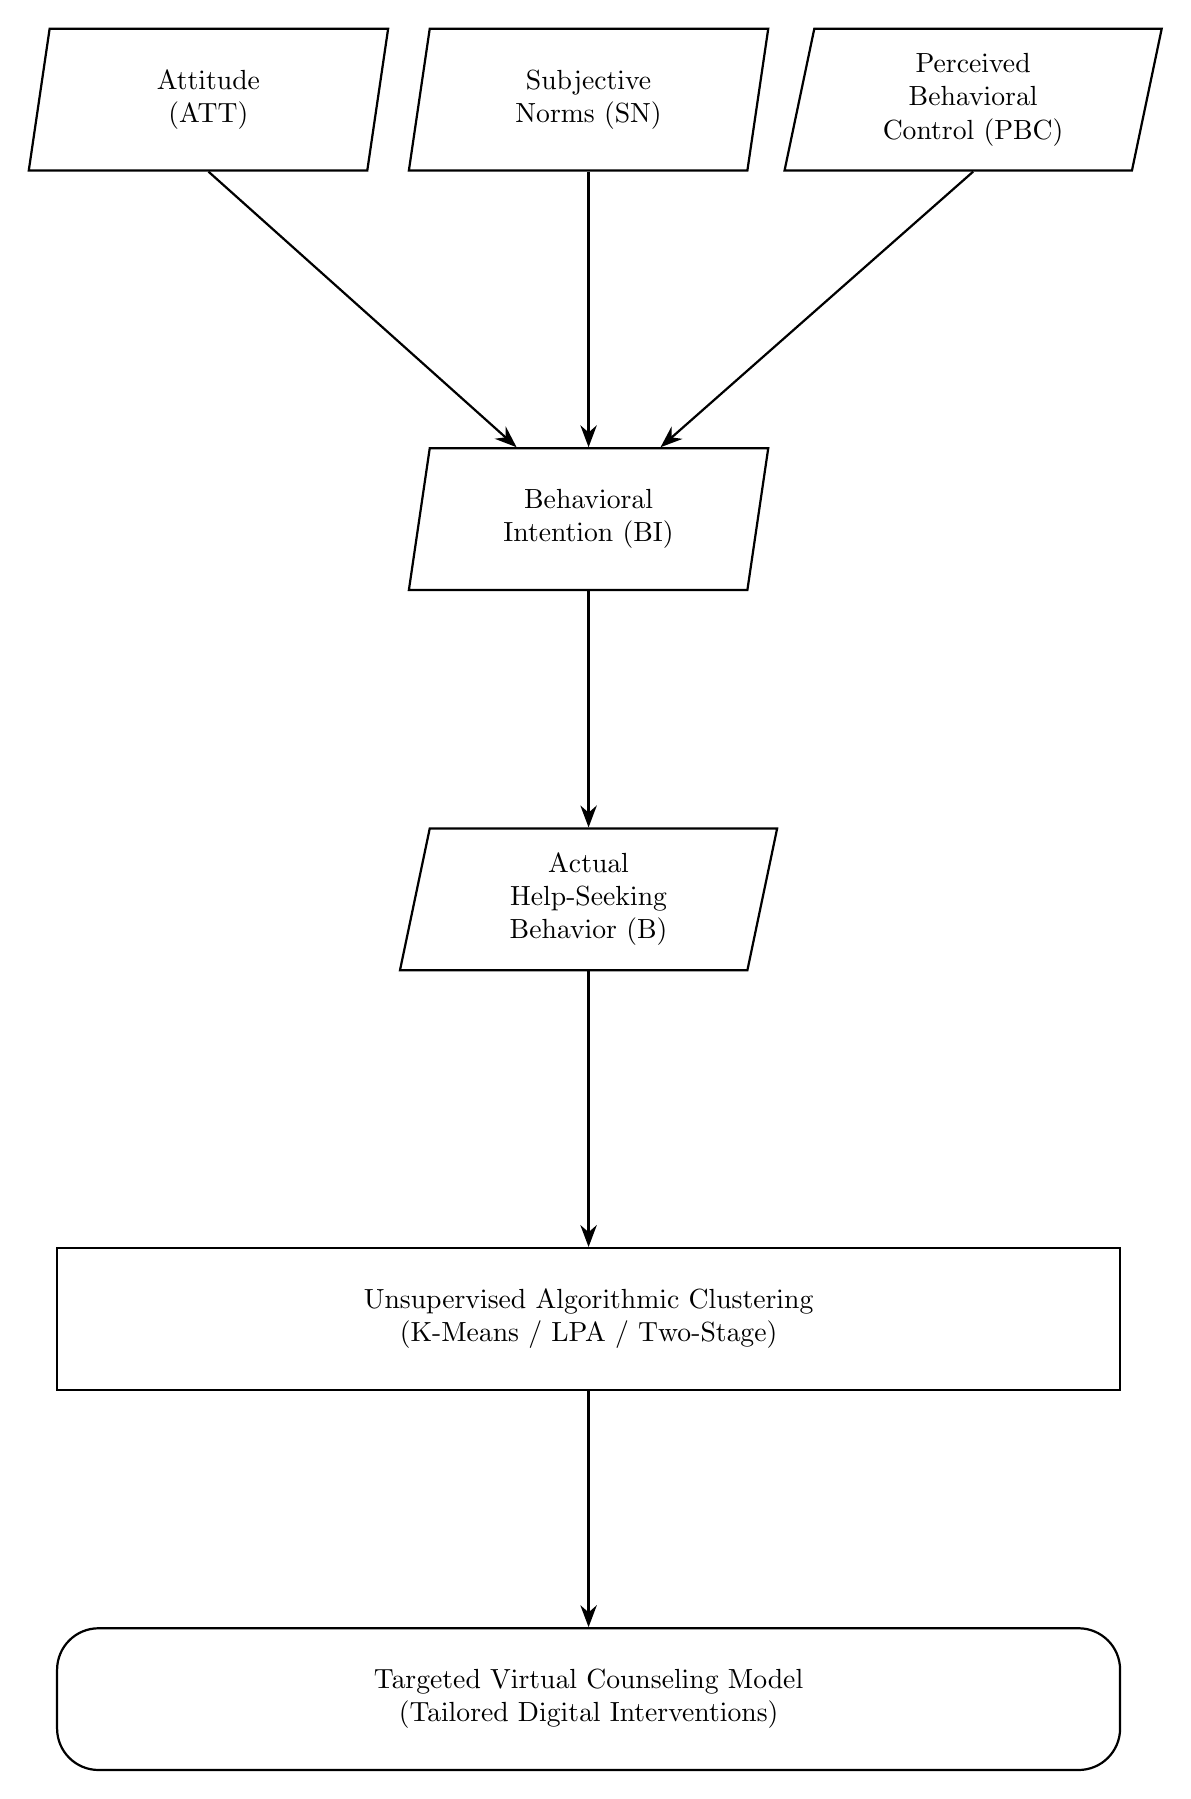
\begin{tikzpicture}[
        node distance=3.5cm and 0.5cm,
        io/.style={trapezium, trapezium left angle=75, trapezium right angle=105, trapezium stretches body=true, draw, thick, align=center, minimum width=4.5cm, text width=3.8cm, minimum height=1.8cm},
        process/.style={rectangle, draw, thick, align=center, minimum width=13.5cm, minimum height=1.8cm},
        terminal/.style={rectangle, rounded corners=15pt, draw, thick, align=center, minimum width=13.5cm, minimum height=1.8cm},
        arrow/.style={-{Stealth[scale=1.2]}, thick}
    ]
    
    % Level 1: TPB Predictors (Data Inputs)
    \node[io] (att) {Attitude \\ (ATT)};
    \node[io, right=of att] (sn) {Subjective \\ Norms (SN)};
    \node[io, right=of sn] (pbc) {Perceived \\ Behavioral \\ Control (PBC)};
    
    % Level 2: Intention (Intermediate Input)
    \node[io, below=3.5cm of sn] (bi) {Behavioral \\ Intention (BI)};
    
    % Level 3: Behavior (Intermediate Input)
    \node[io, below=3cm of bi] (b) {Actual \\ Help-Seeking \\ Behavior (B)};
    
    % Level 4: Clustering (Algorithmic Process)
    \node[process, below=3.5cm of b] (cluster) {Unsupervised Algorithmic Clustering \\ (K-Means / LPA / Two-Stage)};
    
    % Level 5: Outcome (Terminal / End State)
    \node[terminal, below=3cm of cluster] (model) {Targeted Virtual Counseling Model \\ (Tailored Digital Interventions)};
    
    % Connecting Arrows (Level 1 to 2 - Diagonal Funnel)
    \draw[arrow] (att.south) -- (bi.north west);
    \draw[arrow] (sn.south) -- (bi.north);
    \draw[arrow] (pbc.south) -- (bi.north east);
    
    % Connecting Arrows (Level 2 to 3)
    \draw[arrow] (bi.south) -- (b.north);
    
    % Connecting Arrows (Level 3 to 4)
    \draw[arrow] (b.south) -- (cluster.north);
    
    % Connecting Arrows (Level 4 to 5)
    \draw[arrow] (cluster.south) -- (model.north);
    
    \end{tikzpicture}
    \caption{5-Step Analytical Framework Connecting TPB Progression to Algorithmic Outcomes}
    \label{fig:framework}
    \vspace*{\fill}
\end{figure}
\clearpage

\section{Sampling and Secondary Data Collection}
This study will utilize a secondary dataset comprising $N=250$ responses, previously collected as part of a broader, collaborative multi-disciplinary research initiative. The primary data collection targeted parents and primary caregivers of children formally diagnosed with Autism Spectrum Disorder (ASD) in Malaysia. The provided dataset consists of responses to the digital survey instrument utilizing a 5-point Likert scale, adapted to measure the core constructs of the Theory of Planned Behavior (TPB): Attitude, Subjective Norms, and Perceived Behavioral Control (PBC), alongside logistical variables such as geographic accessibility. The methodological focus of this thesis officially begins post-data collection, encompassing the data pre-processing, latent variable extraction, and algorithmic clustering phases.

\section{Data De-identification and Ethical Compliance}
To ensure strict adherence to institutional ethical guidelines regarding human subjects and data privacy, the primary research team will execute a Safe Harbor de-identification protocol prior to the dataset hand-off \citep{Vayena2018_97, WorldHealthOrganization2021_86}. This protocol guarantees the absolute removal of all Personally Identifiable Information (PII) from the $N=250$ dataset, including but not limited to respondent names, email addresses, phone numbers, IP addresses, and exact geographical coordinates. 

Consequently, the secondary dataset utilized in this thesis will consist exclusively of anonymized, numerical, and categorical codes. By ensuring that the computational analysis is performed solely on a fully de-identified matrix, this study bypasses the risks associated with primary data breaches, thereby remaining in full compliance with standard academic ethics board regulations for secondary data analysis \citep{OrganisationforEconomicCooperationandDevelopment2022_81}.

\section{Research Instrument (CSI-PASD)}
Data will be collected using the Bilingual Autism Caregiver Support Instrument (CSI-PASD). The instrument is structured into four primary sections to capture both demographic contexts and psychological variables, as outlined in Table \ref{tab:instrument}.

\begin{table}[H]
    \centering
    \linespread{1.5}\selectfont
    \caption{Structure of the CSI-PASD Instrument}
    \vspace{0.2cm}
    \begin{tabular}{llp{6.5cm}}
        \toprule
        \textbf{Section} & \textbf{Format / Scale} & \textbf{Variables Measured} \\
        \midrule
        \textbf{Section 1} & Binary (Yes/No) & Screening \& Consent (Primary caregiver in Malaysia). \\
        \addlinespace
        \textbf{Section 2} & Categorical & Demographic Data (State of Residence, B40/M40/T20 Income, Child's Severity Level). \\
        \addlinespace
        \textbf{Section 3} & 5-point Likert Scale & Psychological TPB Domains (Attitude, Subjective Norm, Perceived Behavioral Control, Behavioral Intention, Help-Seeking Behavior). \\
        \addlinespace
        \textbf{Section 4} & Open-Ended Text & Qualitative narratives regarding systemic barriers and resilience. \\
        \bottomrule
    \end{tabular}
    \label{tab:instrument}
\end{table}

\section{Validity and Reliability}
To ensure the rigour of the CSI-PASD instrument prior to data collection, Face and Content Validity will be evaluated by a specialized three-expert panel. The composition of this panel and their respective evaluation criteria are detailed in Table \ref{tab:expert_panel}.

\begin{table}[H]
    \centering
    \linespread{1.5}\selectfont
    \caption{Composition of the Expert Validation Panel for Face and Content Validity}
    \vspace{0.2cm}
    \begin{tabular}{llp{7cm}}
        \toprule
        \textbf{Panel Member} & \textbf{Field of Expertise} & \textbf{Primary Validation Focus} \\
        \midrule
        Expert 1 & Statistics \& Psychometrics & Construct validity, PLS-SEM algorithmic assumptions, and scale reliability (AVE, CR, HTMT thresholds). \\
        \addlinespace
        Expert 2 & Clinical Psychology & Clinical accuracy of ASD terminology and psychological constructs within the TPB framework. \\
        \addlinespace
        Expert 3 & Social Science Research & Cultural appropriateness, questionnaire phrasing, and logistical relevance for the Malaysian demographic. \\
        \bottomrule
    \end{tabular}
    \label{tab:expert_panel}
\end{table}

Following data collection, Construct Validity will be mathematically verified utilizing Partial Least Squares Structural Equation Modeling (PLS-SEM). The strict statistical thresholds utilized for model validation are summarized in Table \ref{tab:validity_thresholds}.

\begin{table}[H]
    \centering
    \linespread{1.5}\selectfont
    \caption{Statistical Thresholds for Construct Validity and Reliability}
    \vspace{0.2cm}
    \begin{tabular}{llc}
        \toprule
        \textbf{Metric} & \textbf{Validation Purpose} & \textbf{Acceptance Threshold} \\
        \midrule
        Composite Reliability (CR) & Internal Consistency & $> 0.70$ \\
        \addlinespace
        Cronbach's Alpha ($\alpha$) & Internal Consistency & $> 0.70$ \\
        \addlinespace
        Average Variance Extracted (AVE) & Convergent Validity & $> 0.50$ \\
        \addlinespace
        Heterotrait-Monotrait Ratio (HTMT) & Discriminant Validity & $< 0.90$ \\
        \bottomrule
    \end{tabular}
    \label{tab:validity_thresholds}
\end{table}

\section{Data Pre-processing and Bias Testing}
Prior to executing the primary structural equation modeling and algorithmic clustering, the dataset will undergo rigorous pre-processing to ensure data integrity and mathematically eliminate respondent bias.
First, the dataset will be cleaned to address missing values and unengaged responses (e.g., straight-lining, where a respondent provides the exact same Likert response across all items). Responses exhibiting severe unengaged patterns will be excluded to prevent algorithmic distortion.
Next, the normality of the data distribution will be evaluated using Skewness and Kurtosis thresholds. Because social science survey data often violates strict multivariate normality, verifying the distribution justifies the subsequent use of PLS-SEM, which is highly robust against non-normal data.
Finally, to address the quantitative risk of respondent bias inherent in self-reported questionnaires, \textbf{Common Method Bias (CMB)} will be evaluated using \textbf{Harman's Single Factor Test}. All items will be loaded into an unrotated exploratory factor analysis. If the total variance extracted by a single factor is less than the critical threshold of 50\%, it mathematically confirms that no single latent factor (such as temporary respondent mood or survey fatigue) artificially inflates the variance, thereby ensuring the dataset is unbiased and ready for K-Means processing.

\section{Latent Variable Estimation (PLS-SEM)}
Because survey data is ordinal, it mathematically violates the continuity assumptions of distance-based clustering. To resolve this, Partial Least Squares Structural Equation Modeling (PLS-SEM) will first be utilized \citep{Hair2021}. By validating internal consistency and construct validity, PLS-SEM allows for the extraction of \textbf{Latent Variable Scores}. This process transforms ordinal variables into standardized, continuous latent vectors ($\mu = 0, \sigma = 1$), providing a mathematically robust input matrix for the subsequent clustering algorithms.

\section{Comparative Clustering Algorithms}

\subsection{Model 1: K-Means Clustering (Distance-Based)}
K-Means is a non-hierarchical, deterministic algorithm that partitions observations into $k$ distinct sets $S = \{S_1, S_2, \dots, S_k\}$. It operates by minimizing the within-cluster sum of squares (WCSS), defined as:
\begin{equation}
    \text{WCSS} = \sum_{j=1}^{k} \sum_{x_i \in S_j} ||x_i - \mu_j||^2
\end{equation}
where $x_i$ represents the latent psychometric vector of a caregiver, and $\mu_j$ is the centroid of cluster $S_j$. K-Means utilizes "hard assignment," making it computationally efficient and highly effective at minimizing spatial variance \citep{Hastie2009}.

\subsection{Model 2: Latent Profile Analysis (Probability-Based)}
Unlike K-Means, Latent Profile Analysis (LPA) assumes that the caregiver population is a mixture of underlying, unobserved probability distributions. LPA utilizes a Gaussian Mixture Model (GMM) to estimate the probability that a specific caregiver belongs to a certain latent profile. The model assumes a probability density function:
\begin{equation}
    f(x_i) = \sum_{j=1}^{k} \pi_j \phi(x_i | \mu_j, \Sigma_j)
\end{equation}
where $\pi_j$ is the mixing proportion of profile $j$, and $\phi$ is the multivariate normal density with mean vector $\mu_j$ and covariance matrix $\Sigma_j$. LPA provides "soft assignment," acknowledging the probabilistic nuances of human psychology.

\subsection{Model 3: Two-Stage Clustering}
The Two-Stage Clustering approach integrates both hierarchical and partitioning methods to overcome the limitations of isolated algorithms. In the first stage, a hierarchical algorithm (such as Ward's method) is employed to iteratively construct a dendrogram and determine the optimal number of clusters ($k$). In the second stage, the centroids identified by the hierarchical method are used as the initial, non-random "seed" values for a K-Means algorithm, potentially leading to more stable and replicable final assignments.


\section{Model Evaluation Criteria}
To declare the mathematically optimal model for ASD caregiver profiling, the outputs of all three algorithms will be subjected to rigorous comparative evaluation.

For the distance-based models (K-Means, Two-Stage), the primary metric will be the \textbf{Silhouette Score}, which measures cluster cohesion versus separation:
\begin{equation}
    s(i) = \frac{b(i) - a(i)}{\max\{a(i), b(i)\}}
\end{equation}
where $a(i)$ is the mean intra-cluster distance and $b(i)$ is the mean nearest-cluster distance. A score approaching $+1$ indicates excellent cluster separation.

For the probability-based model (LPA), model fit will be evaluated using Information Criteria, specifically the \textbf{Bayesian Information Criterion (BIC)} and \textbf{Akaike Information Criterion (AIC)}:
\begin{equation}
    \text{BIC} = -2 \ln(\hat{L}) + p \ln(n)
\end{equation}
where $\hat{L}$ is the maximized likelihood of the model and $p$ is the number of estimated parameters. Models with lower BIC values will be prioritized, penalizing unnecessary algorithmic complexity to prevent overfitting.

\section{Post-Clustering Profile Interpretation}
Following the mathematical selection of the optimal clustering model, the final phase of the methodology involves transforming the statistical groupings (e.g., Cluster 1, Cluster 2) into human-interpretable caregiver profiles. This will be achieved by conducting Cross-Tabulation and Analysis of Variance (ANOVA/Chi-Square) to map the psychological TPB clusters against the demographic variables collected in Section 2 of the CSI-PASD (Income, State of Residence, Child's Severity Level). By correlating the statistical clusters with socio-demographic contexts, the research can identify holistic, actionable personas (e.g., "The Overwhelmed Rural Caregiver") to inform targeted counseling recommendations.


\bibliographystyle{apalike}
\bibliography{references}

\chapter*{Research Gantt Chart}
\addcontentsline{toc}{chapter}{Research Gantt Chart} % Adds this to the Table of Contents

The following Gantt chart outlines the proposed timeline for the completion of this Master by Research project, spanning from the initial Defense of Research Proposal (DRP) through the phases of secondary data collection, algorithmic processing, manuscript preparation, and final thesis submission.

% --- IMAGE PLACEHOLDER: GANTT CHART ---
% Note: You must place your Excel screenshot named 'gantt_chart.png' inside the 'figures' folder.
\begin{figure}[H]
    \centering
    % \includegraphics[width=1.0\textwidth]{figures/gantt_chart.png}
    \caption{Proposed Project Timeline and Milestones.}
    \label{fig:gantt}
\end{figure}
% --------------------------------------


\end{document}
